\documentclass[12pt]{article}

\usepackage{sbc-template}
\usepackage{graphicx,url}
\usepackage[utf8]{inputenc}
\usepackage[brazil]{babel}
%\usepackage[latin1]{inputenc}  
     
\sloppy

\title{Arquitetura para Detecção de Postura Inadequada para Prevenção de Hipercifose Utilizando Arduino Lilypad}

\author{Ênio J. F. Júnior\inst{1}, Jonas S. Ramos\inst{1}, Hiel A. Rocha\inst{1} }

\address{Bacharelado em Ciência da Computação -- Instituto de Educação Superior\\ de Brasília
  (IESB) -- Brasília -- DF -- Brazil
  \email{\{juniorr452,jjonasramos\}@gmail.com,  hielrocha@outlook.com.br}
}

\begin{document} 

\maketitle

\begin{abstract}
  This paper presents an architecture for incorrect posture detection using Arduino based components and fuzzy logic. The goal is to warn the user if his posture is not correct to prevent hypercifosis.
\end{abstract}
     
\begin{resumo} 
  Este artigo apresenta uma arquitetura para detecção de postura incorreta com o uso de componentes de Arduino e lógica fuzzy. O objetivo é notificar o usuário se a postura dele estiver incorreta para prevenir a hipercifose
\end{resumo}

\section{Introdução}

Ter uma postura correta é fundamental para evitar problemas na coluna e ter uma boa qualidade de vida. De acordo com \cite{cru:17}, segundo a OMS, a dor nas costas atinge cerca de 80\% da população mundial, sendo um dos motivos para isso a postura inadequada. Já outro levantamento aponta que dor nas costas foi uma das principais causas para afastamento no trabalho \cite{ig:17}.  

Além de, eventualmente, causar dor nas costas, a má postura pode de causar deformidades na coluna, como, por exemplo, a hipercifose, um agravamento da curvatura natural da coluna. 

\begin{figure}[ht]
\centering
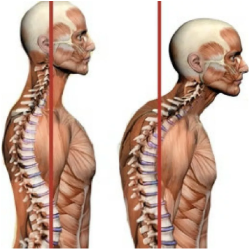
\includegraphics{fig4.png}
\caption{Cifose (esquerda) e hipercifose (direita) (Imagem: Vickyfisio)}
\label{fig:example4}
\end{figure}

Segundo Vidal, a cifose é “uma curvatura normal da coluna vertebral” \cite{vidal:17}. Já a hipercifose é “uma alteração nessa região da coluna que leva a um aumento da cifose normal, deixando os ombros projetados para frente e o dorso arredondado” \cite{vidal:17}. Uma das causas é a má postura, que pode acarretar dor nas costas.

Neste artigo, é proposto uma arquitetura de detecção de postura inadequada com o uso de sensores, a fim de notificar o usuário quando ela estiver inadequada para a prevenir a hipercifose.

\section{Trabalhos Correlatos}
Em 2017, a camisa inteligente \textit{10ELEVEN9} \cite{colorfy:17} foi apresentada no site de financiamento coletivo \textit{Kickstarter}. A proposta era de proporcionar diversas funcionalidades com uma única peça vestível. Dentre elas, pode-se destacar o uso de um sensor de acelerômetro para detectar a postura do usuário e informá-lo, caso ela seja considerada incorreta. Por estar integrado junto ao sensor de batimentos cardíacos, o componente fica localizado na região peitoral. A descrição do projeto não especifica qual o algoritmo utilizado para considerar a postura correta ou incorreta.

\begin{figure}[ht]
\centering
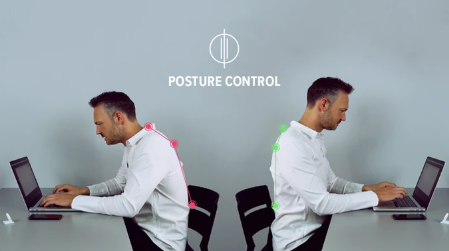
\includegraphics{fig2.png}
\caption{Sistema de controle de postura do 10ELEVEN9}
\label{fig:example2}
\end{figure}

O trabalho \textit{Posture Correction with Wearable Electronics} \cite{rubow:08} teve, como objetivo, identificar a postura inadequada do usuário. Os componentes utilizados nesse projeto foram: Arduino Lilypad, dois acelerômetros e um módulo \textit{bluetooth} para receber dados dos sensores.

Quanto ao posicionamento dos componentes e algoritmos do projeto, os acelerômetros são posicionados na região dos ombros e o cosseno do ângulo entre os vetores gravitacionais dos sensores são calculados. O usuário é notificado por um som pelo módulo \textit{bluetooth} quando a diferença entre eles passa de um determinado limiar.

O estudo concluiu que o uso do módulo \textit{bluetooth}, bem como a bateria e regulador de voltagem, não seriam adequados, pois esses componentes não foram projetados especificamente para roupas. Inclusive, tais componentes precisaram ser acoplados a uma placa para então ser costurado na roupa, o que deixou o protótipo com aspecto esquisito.

Este projeto envolve utilizar os componentes de acelerômetro e o \textit{buzzer}, projetados especificamente para integração com tecidos, para captar detectar e notificar o usuário se sua postura está adequada ou não.

\section{O Projeto}

\subsection{Tecnologias}

Para construir uma arquitetura de detecção de postura incorreta, este trabalho fará uso dos seguintes softwares e componentes de hardware:

\begin{itemize}
    \item Arduino IDE;
    \item Arduino Lilypad;
    \item Acelerômetro;
    \item \textit{Buzzer}.
\end{itemize}

O Arduino IDE é um software que permite escrever programas para serem executados no dispositivo Arduino Lilypad. O sensor de acelerômetro e o \textit{buzzer} possibilitam obter os dados necessários para saber a postura e notificar o usuário, caso ela não esteja adequada.

\subsection{Arquitetura}

Um modelo da arquitetura proposta pode ser visualizado na figura a seguir, que mostra a ligação entre o Lilypad e seus componentes.

\begin{figure}[ht]
\centering
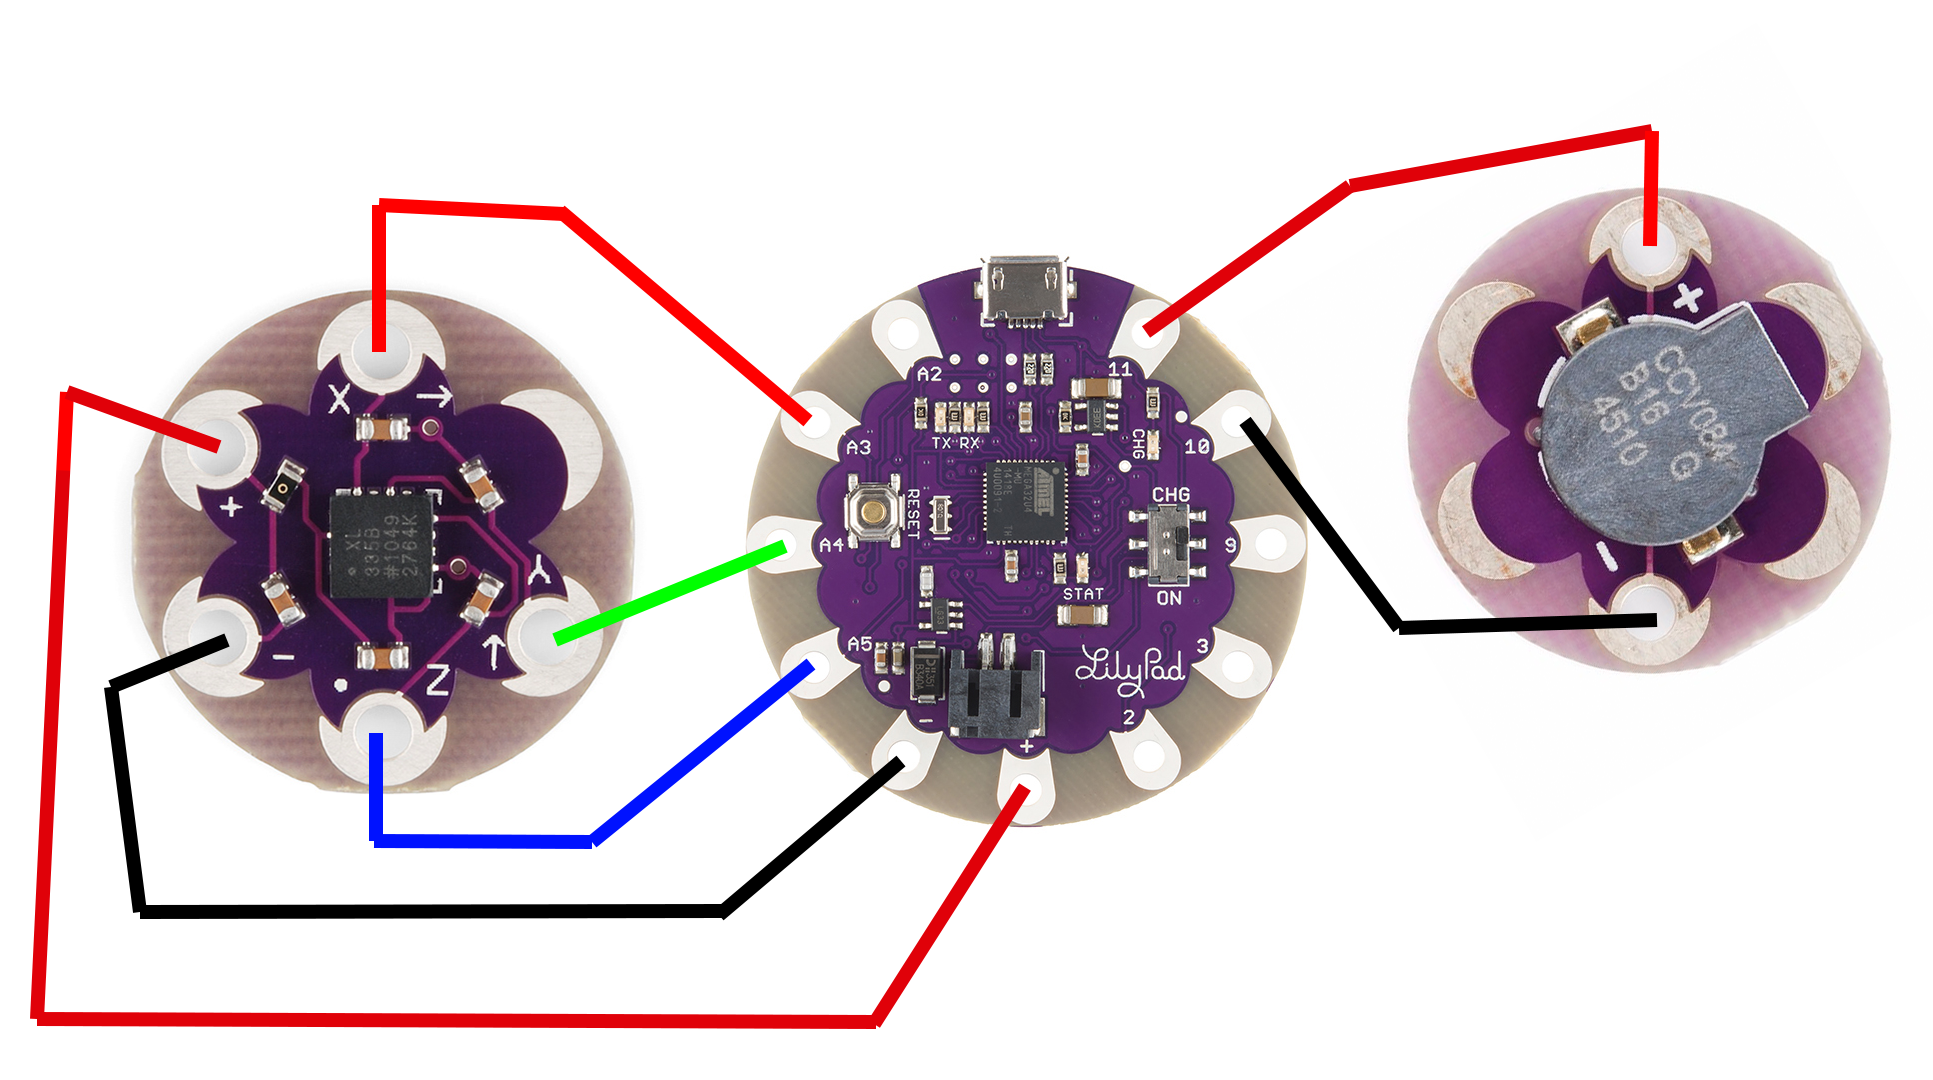
\includegraphics[width=.8\textwidth]{diagrama_conexao.png}
\caption{Arquitetura proposta. O acelerômetro (esquerda), Lilypad USB (meio) e \textit{buzzer} (direita).}
\label{fig:example3}
\end{figure}

O acelerômetro será costurado perto do pescoço para detectar a inclinação da região. A partir disso, será elaborado um algoritmo, cujo o código será executado pelo Lilypad, para identificar se a inclinação do pescoço é ou não ideal para a postura em um determinado período de tempo e produzir som através do \textit{buzzer} para notificar o usuário de que sua postura está incorreta.

Sobre o sistema, sãu utilizadas 3 variáveis: postura, \textit{sombuzzer} e \textit{delay}. A postura é o valor de um dos eixos do acelerômetro para verificação da postura do usuário. O \textit{sombuzzer} é uma variável do tipo \textit{int} que representa o volume do \textit{buzzer}. Já a variável \textit{delay} é o intervalo entre os apitos do \textit{buzzer}. Os seguintes conjuntos \textit{fuzzy} são utilizados para avaliação da postura:\newline

\begin{figure}[ht]
    \centering
    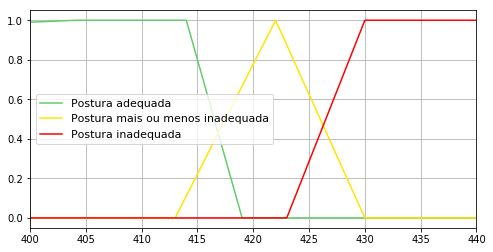
\includegraphics[width=.7\textwidth]{download.png}
    \caption{Conjuntos \textit{fuzzy} para verificação de postura inadequada}
    \label{fig:fuzzy1}
\end{figure}

\break

O sistema de inferência \textit{fuzzy} possui as seguintes regras:

\begin{itemize}
    \item Se a postura estiver MAIS OU MENOS INADEQUADA, então \textit{sombuzzer} é igual a 100 e \textit{delay} é igual a 10;
    \item Se a postura estiver INADEQUADA, então \textit{sombuzzer} é igual a 1500 e \textit{delay} é igual a 50;
\end{itemize}

Para defuzificação, é usado o conjunto \textit{fuzzy} com maior grau de pertinência para obter o valor das variáveis \textit{sombuzzer} e \textit{delay}.

\bibliographystyle{sbc}
\bibliography{sbc-template}

\end{document}
